\chapter{Song-Havlin-Makse self-similar model}

%\resp{Franco Aquistapace Tagua}

\section{Introduction and methods}
 
The work by Song, Havlin and Makse \cite{song2006origins} aims to explain the characteristic features of empirical scale--free fractal and non--fractal networks by means of a single growth model, that has the concept of renormalisation at its core. More specifically, the proposed growth mechanism works as the inverse of the renormalisation procedure. The goal of this task is then to reproduce their growth and renormalisation procedures, and to recover the characteristic behaviour of fractal and non--fractal networks through relevant descriptors. 

When performing the growth process of a network, each existing node is considered as a future hub. For a node with degree $k$, $mk$ offspring nodes are attached to it at each growth step. Then, each edge between two of the original nodes is removed with probability $p=1-e$, and replaced by an edge between two of their offspring. The parameter $e$ then controls the hub--hub attraction/repulsion behaviour of the network. Mode I growth, given by $e\rightarrow1$, leads to hub--hub attraction and a non--fractal topology. Meanwhile, Mode II growth, given by $e\rightarrow0$, leads to hub--hub repulsion and a fractal network. This growth process is referred to as the minimal model. The renormalisation of a network is then done as described in the source material, by covering its $N$ nodes with $N_B(L_B)$ boxes, where the maximum shortest path between any two nodes in a box must be $L_B$.

For each case $e=1.0, 0.8$, a set of 10 graphs is generated with the minimal model. In all cases, the network is initialised as a star graph with $N_{init}=5$ nodes. Then, the growth mechanism is applied $n_{growth}=4$ times, with a growth factor of $m=2$. Once obtained, each graph is then subjected to the normalisation procedure for distances $1\leq L_B\leq32$. Furthermore, for each minimal model graph an uncorrelated version is generated by random swapping of links, while maintaining the degree distribution. The normalisation procedure is also applied to the randomised graphs. Additional details on the methodology can be found in section \ref{sec:SHM_SM} of the Supplementary Material.


\section{Results and discussion}

The correlation profile, $R(k_1,k_2)$, can be used to visualise the correlated topological structure of the minimal model, in comparison to its random uncorrelated counterpart. Fig. \ref{fig:R_k1_k2_comparison} presents the $R(k_1,k_2)$ matrices for both cases $e=1.0, 0.8$. It can be seen that $e=1.0$ leads to hub--hub attraction, while hub--hub repulsion is observed for the case $e=0.8$. This descriptor is however insufficient to define the fractality of a network, as it cannot describe how the topology of the network changes under renormalisation. 

In order to complement this, the scaling relations $N_B(L_B) / N$ and $\mathcal{S}(L_B)$ are estimated for the minimal model graphs, where $\mathcal{S}(L_B)$ is the maximum degree scaling. The results of $N_B(L_B) / N$ and $\mathcal{S}(L_B)$ are presented in Fig. \ref{fig:N_B_and_S_vs_L_B} with respect to $L_B$, for both cases $e=1.0, 0.8$. As in the source material, an exponential decay of both descriptors can be seen for the non--fractal topology resulting in the case $e=1.0$. Meanwhile, the power--law behaviour of fractal networks is observed in both descriptors for the case $e=0.8$. A finite--size effect can be observed for large values of $L_B$, more noticeably for the case $e=1.0$, which appears as a constant value of the scaling relations.

\begin{figure}[!h]
	\begin{center}
	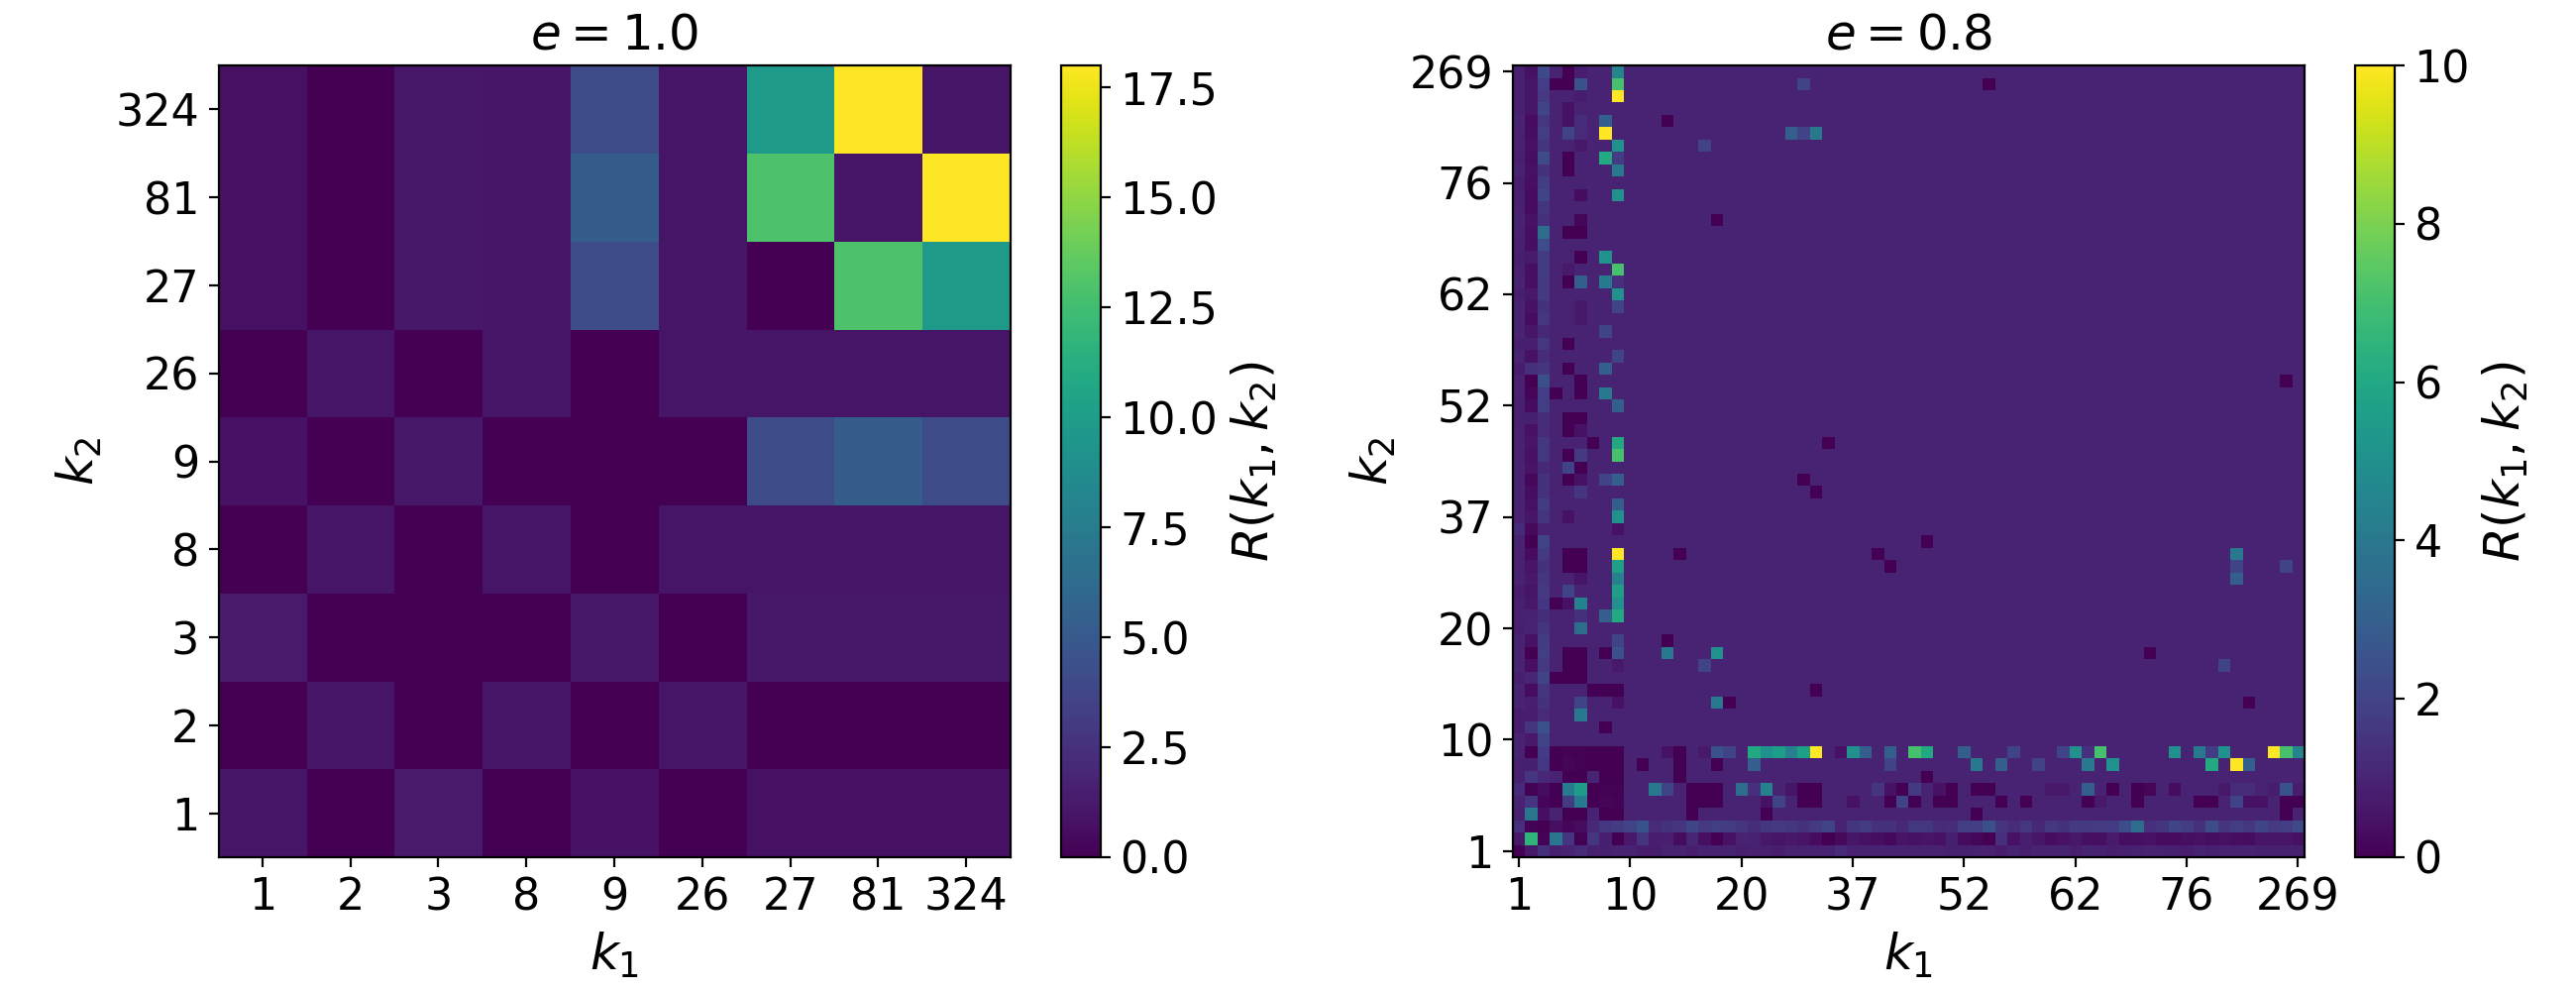
\includegraphics[scale=0.46]{./images/task_6/R_k1_k2_comparison.png} 
	\end{center}
	\caption{Correlation profile $R(k_1, k_2)$ of networks generated with the minimal model, for the cases $e=1.0$ (left) and $e=0.8$ (right). \\} 
	\label{fig:R_k1_k2_comparison} 
\end{figure}

\begin{figure}[!h]
	\begin{center}
	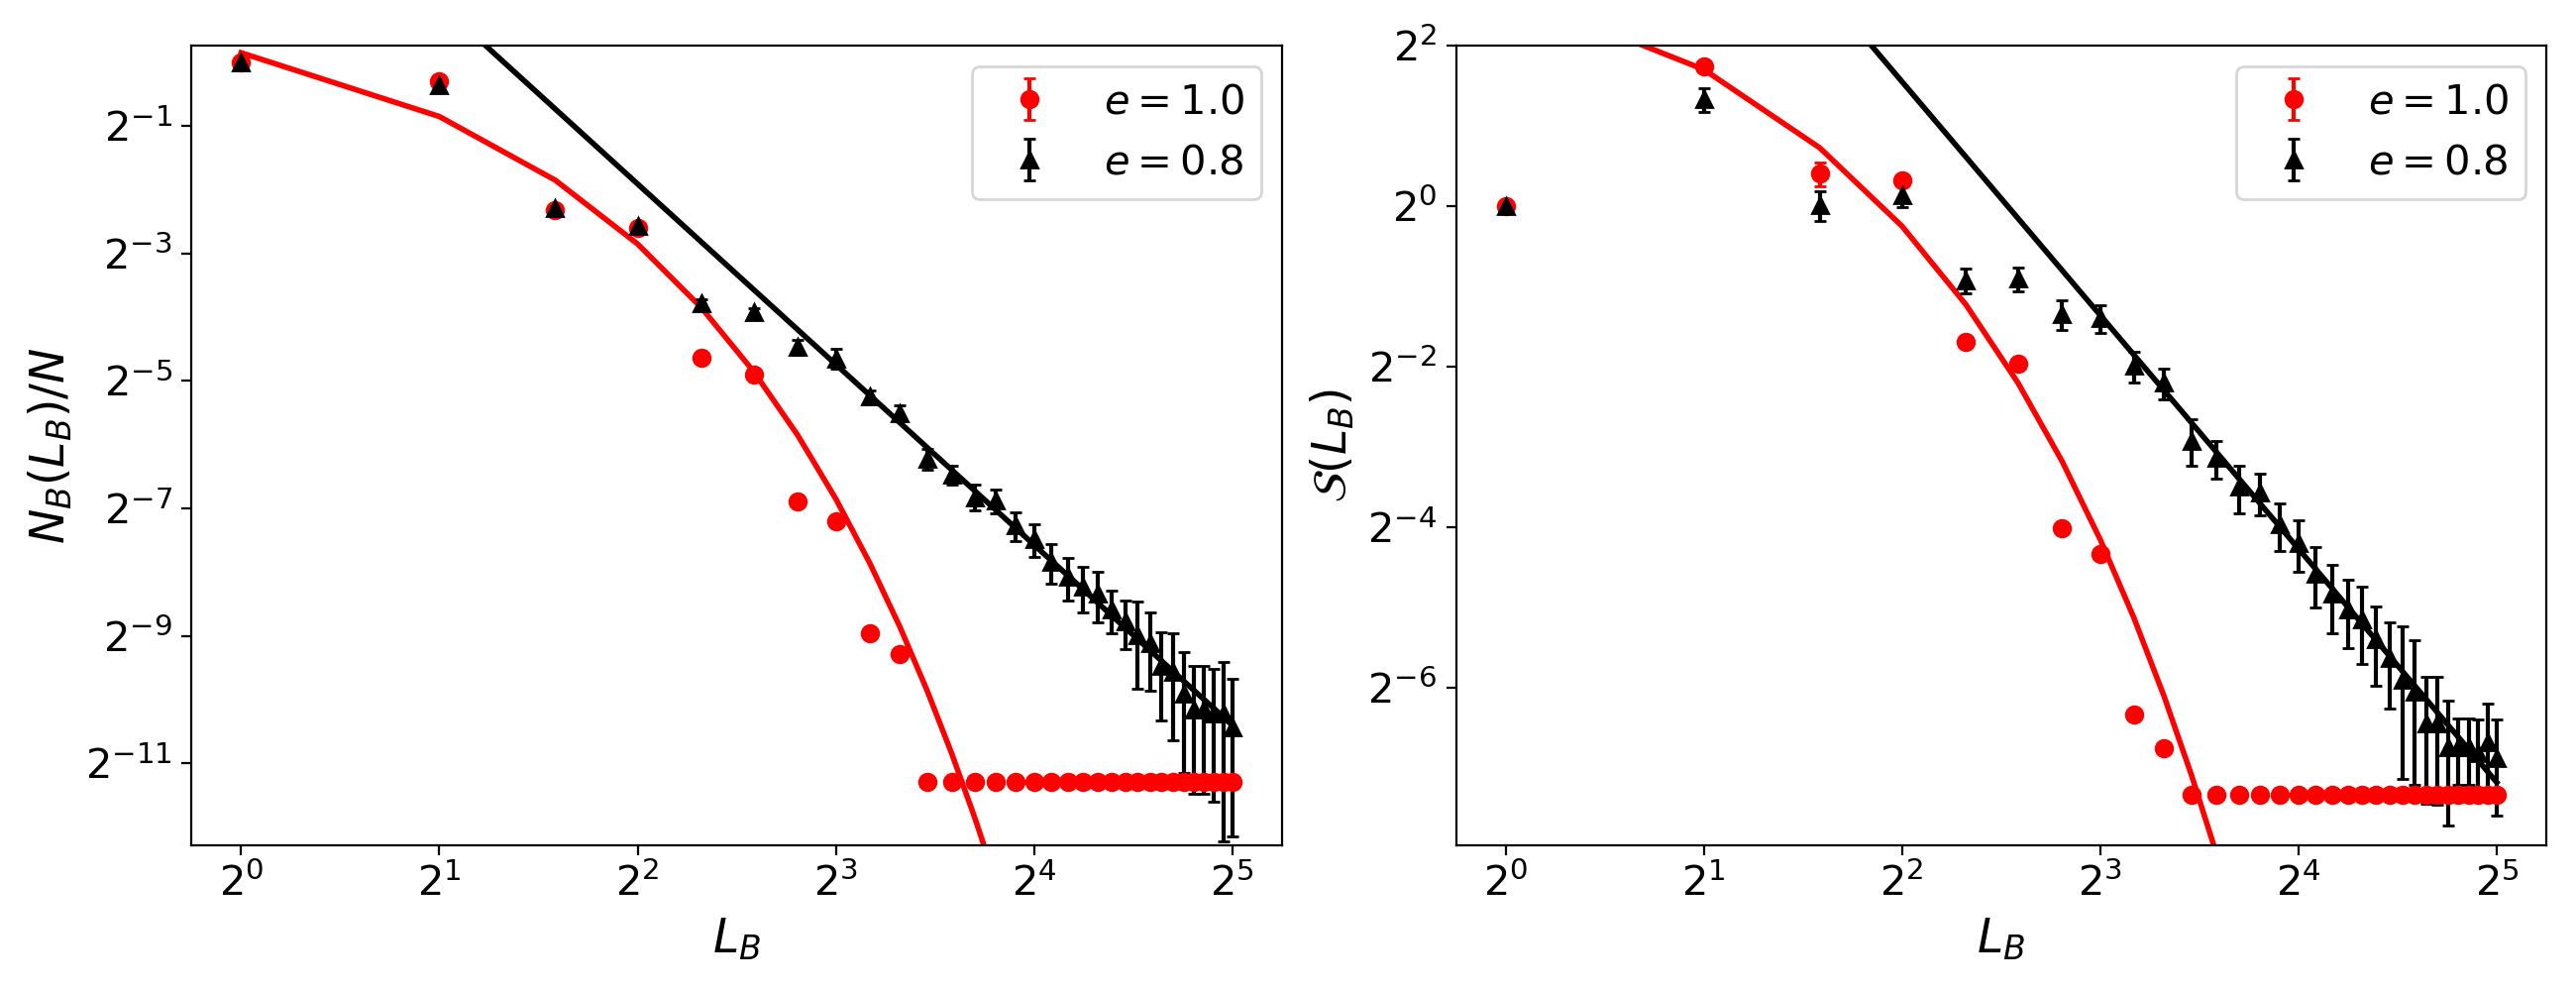
\includegraphics[scale=0.46]{./images/task_6/N_B_and_S_vs_L_B.png} 
	\end{center}
	\caption{Scaling relations $N_B(L_B) / N$ (left) and $\mathcal{S}(L_B)$ (right) with respect to box distance $L_B$. Results are shown for networks generated with the minimal model, for the cases $e=1.0$ and $e=0.8$.\\} 
	\label{fig:N_B_and_S_vs_L_B} 
\end{figure}


%\begin{figure}
%\centering     %%% not \center
%\subfigure[Figure A]{\label{fig:a}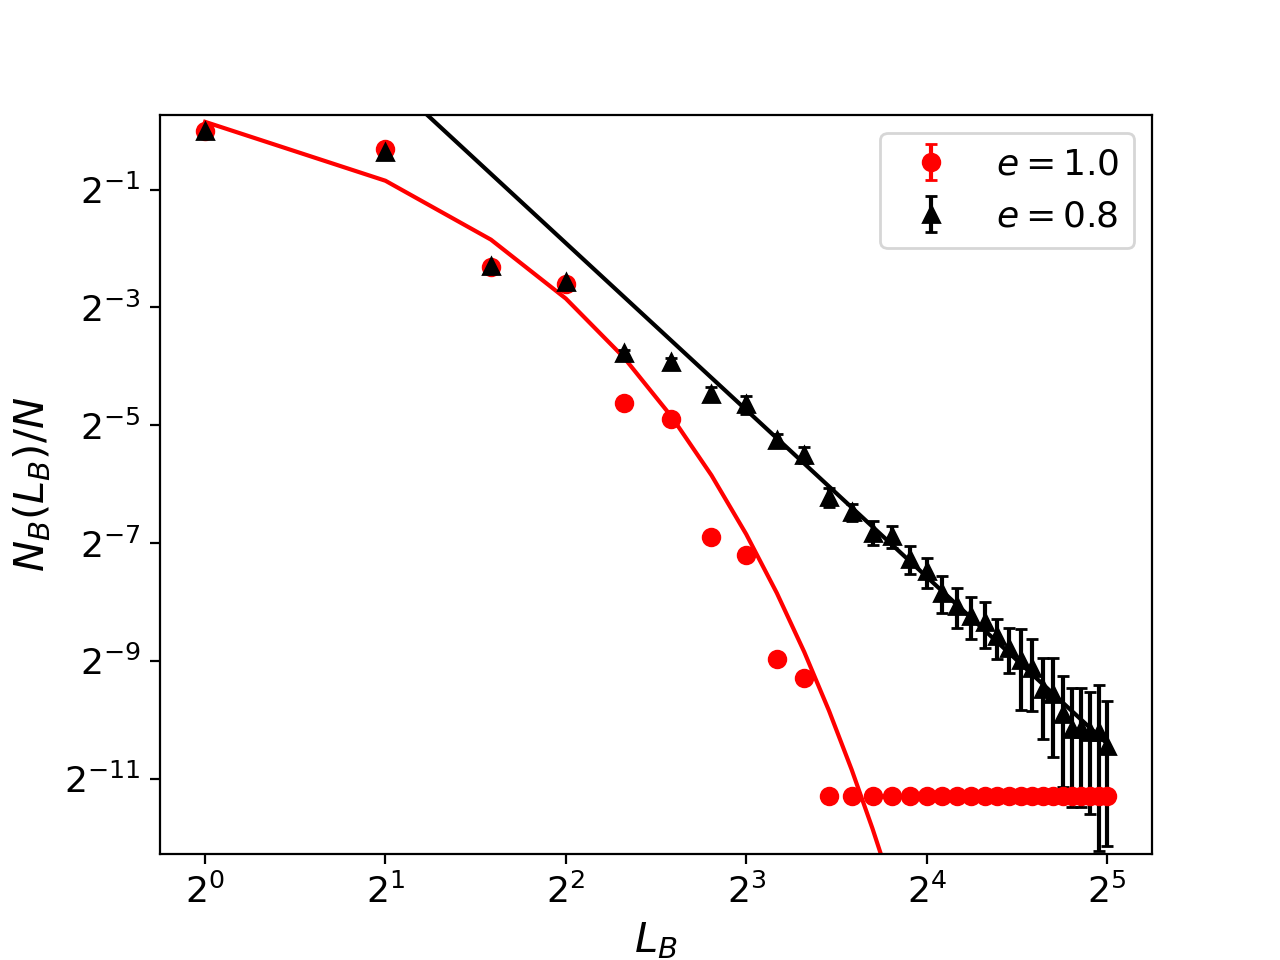
\includegraphics[width=60mm]{./images/task_6/N_B_N_vs_L_B.png}}
%\subfigure[Figure B]{\label{fig:b}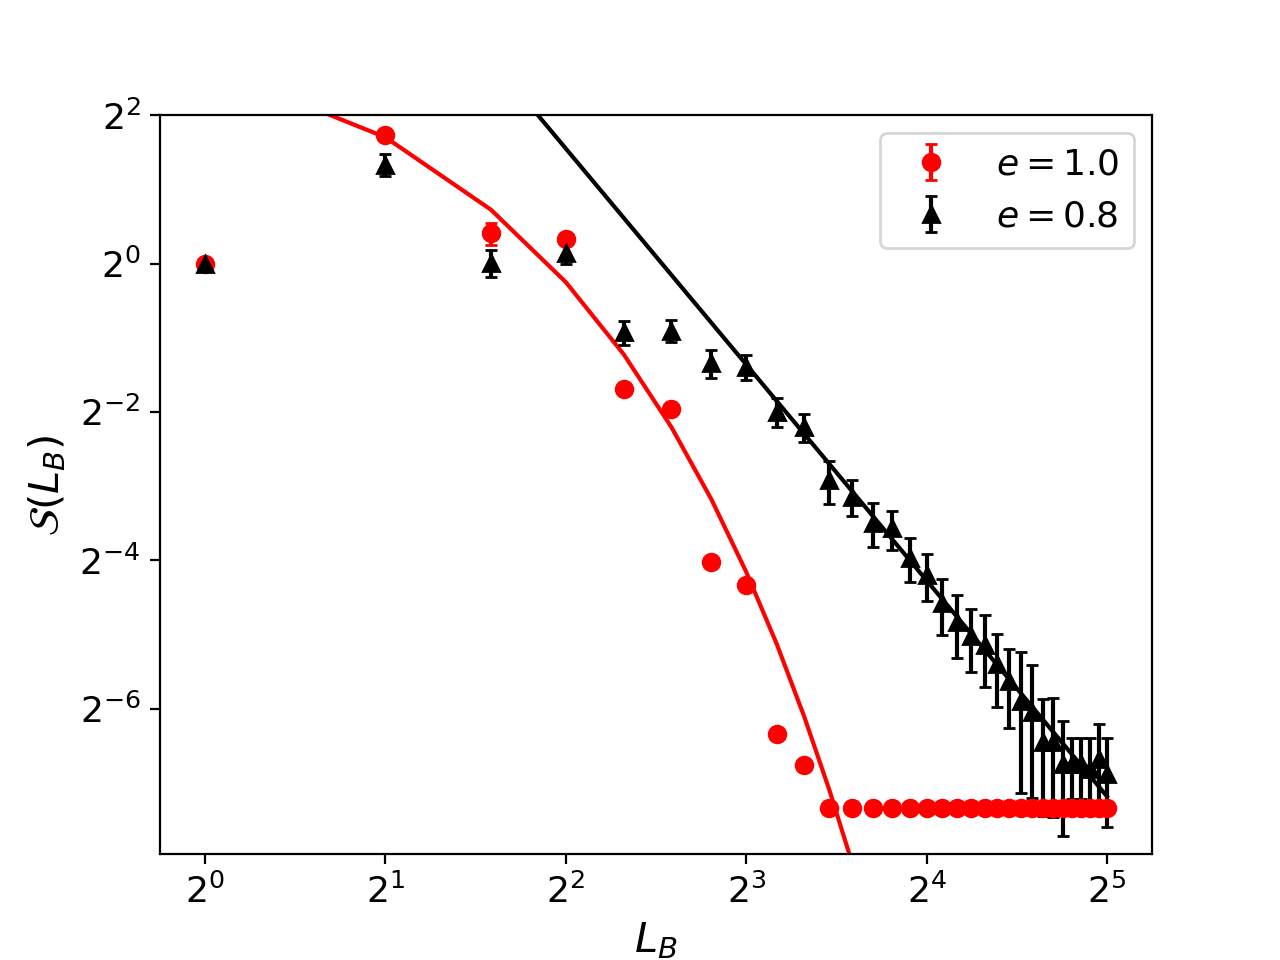
\includegraphics[width=60mm]{./images/task_6/S_vs_L_B.png}}
%\caption{my caption}
%\end{figure}

%\lipsum[2-4]


\newpage